% !TEX program = pdflatex+makeindex+bibtex
% !TEX encoding = UTF-8 Unicodede_ch

% created by Simon Schälli <simon.schaelli@kantiwattwil.ch>
% v1.0 ursprüngliche Version
% v1.1 2015-10-22 mit Titelbild
% v1.2 2016-09-30 aufgeräumt
% v1.3 2016-10-16 Layoutfehler behoben

%======================================================================%
%=== Dokument auf häufige Fehler überprüfen                         ===%
%======================================================================%
\RequirePackage[l2tabu, orthodox]{nag}

%======================================================================%
%=== Dokumentklasse wählen                                          ===%
%======================================================================%
\documentclass[a4paper,openright]{scrreprt}

%======================================================================%
%=== Pakete einbinden                                               ===%
%======================================================================%
\usepackage[utf8]{inputenc}
\usepackage[english]{babel}

% Latin Modern Schriftart
\usepackage{lmodern}
\usepackage[T1]{fontenc}

% Mathematik-Pakete
\usepackage{amsmath}
\usepackage{amssymb}
\usepackage[mathscr]{euscript}

% mathematische Buchstaben als Text
\usepackage{textcomp}

% komfortable Referenzen mit \fref
\usepackage[english]{fancyref}

% Kopf- und Fusszeilen
\usepackage[automark,headsepline]{scrpage2}
\ihead[]{\headmark}
\chead[]{}
\ohead[]{\pagemark}
\ifoot[]{}
\cfoot[\pagemark]{}
\ofoot[]{}
\pagestyle{scrheadings}

% Einfügen von Bildern
\usepackage{graphicx}

% schöne Tabellen
\usepackage{booktabs}

% Tabelleninhalt an Dezimalpunkt ausrichten
\usepackage{dcolumn}
\makeatletter                     % <- hebt Sonderbedeutung von @ auf
\newcolumntype{d}[1]{D{.}{.}{#1}} % <- definiert einen neuen Spaltentyp
\makeatother                      % <- setzt Sonderbedeutung von @ wieder

% Beispieltext
\usepackage{lipsum}

% Hyperlinks in PDF
\usepackage{hyperref}

% Biblatex
\usepackage[
backend=biber,
style=numeric,
sorting=ynt
]{biblatex}
\addbibresource{Bibliography.bib}

% Macros
\usepackage{mymacros}
\usepackage{xargs}

%======================================================================%
%=== Angaben zum Dokument                                           ===%
%======================================================================%

\titlehead{Kantonsschule im Lee \hfill Kalani Fin Kistler\\
Fachschaft Mathematik \hfill Dättnauerstrasse 107\\
Rychenbergstrasse \hfill 8406 Winterthur\\
8400 Winterthur}
\subject{Matura Thesis}
\title{An Exploration of Applied Reinforcement Learning}
\author{\texorpdfstring{Kalani Fin Kistler \\[1cm]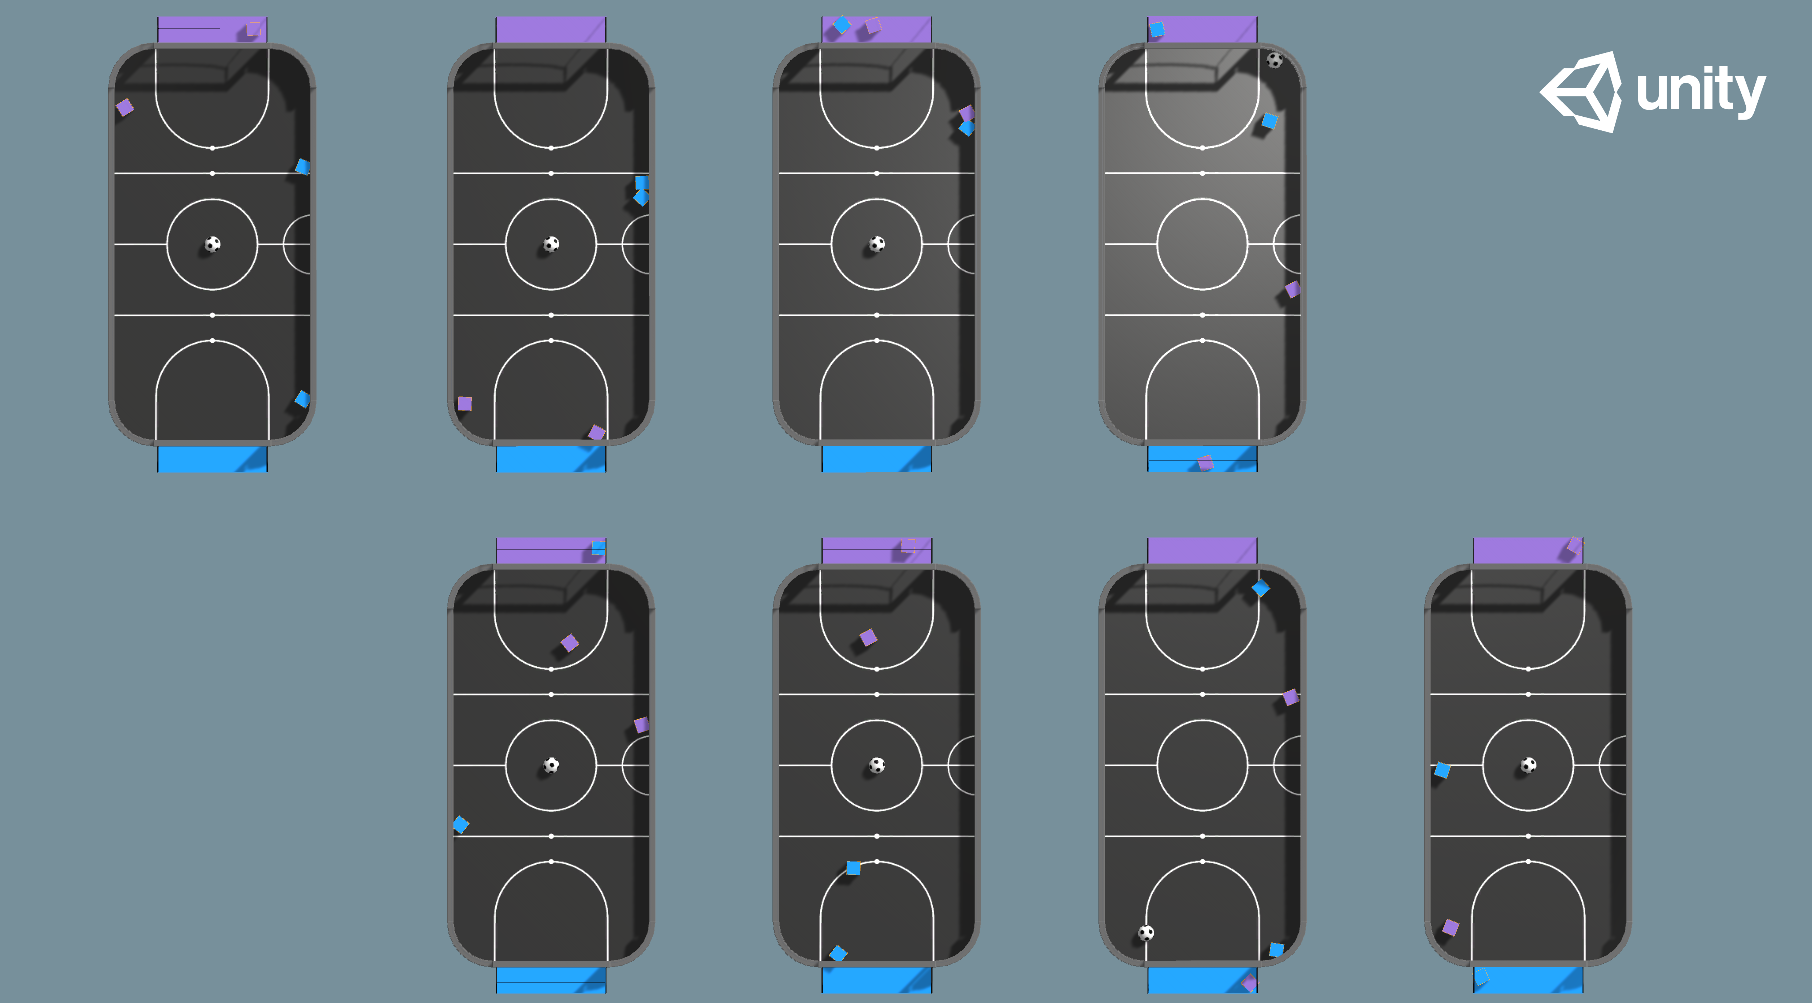
\includegraphics[scale=0.2]{figures/Screenshot from 2020-09-22 23-05-59.png}\\[1cm] {\small Supervisor: Elena Fattorini}}{Kalani Fin Kistler}}
\date{\small xx.xx.20xx}
%======================================================================%
%=== PDF Dokumenteinstellungen                                      ===%
%======================================================================%

\makeatletter
\hypersetup{
	pdftitle={\@title},%
	pdfsubject={\@subject},%
	pdfauthor={\@author},%
	pdfkeywords={},%
	colorlinks,%
	citecolor=black,%
	filecolor=black,%
	linkcolor=black,%
	urlcolor=black}%
\makeatother


%======================================================================%
%=== Beginn des eigentlichen Dokumentes                             ===%
%======================================================================%

\begin{document}

\maketitle % <- Titel setzen
\cleardoublepage
\pagenumbering{roman} % <- römische Seitennummerierung
\tableofcontents % <- Inhaltsverzeichnis
\cleardoublepage % <- neue Seite
\pagenumbering{arabic} % <- arabische Seitennummerierung

% Kapitel einbinden:

\chapter*{NOTES FOR CHAPTER HAND IN ONLY, NOT ON FINAL}
Due to the fact taht I am not yet fammiliar with vectorgraphics and wanted to focus on writing, the figures are temporary stand ins, meant only to convey the content of the final image and not the final image itself.

% !TEX root = ../maturaarbeit.tex
\chapter{Introduction}\label{chap:einleitung}

% !TEX root = ../maturaarbeit.tex
\chapter{Background}\label{chap:theory}
\section{Reinforcement Learning}\label{sec:RL}

Throughout our daily lives we navigate our surroundings, handle social situations and tackle complex tasks. In doing, so we seek to take actions that based on experience or intuition we believe to have the best outcome. We might take these abilities for granted give how natural they are. However, at some point we had to obtain these skills which are so essential in managing our day to day, many through simple trial and error. Reinforcement Learning (RL) seeks to formalize this process of figuring out how to behave based on seeing what produces desirable results and what does not, and adjusting our future actions accordingly. 
Reinforcement Learning is a discipline of machine learning \cite[p. 1]{sutton_reinforcement_2018} , an incredibly broad field which is focused on the self-improvement of computer algorithms by processing data and experience. 
As such it is at the interface between the natural and to us intuitive concept of learning and overwhelmingly rigid and numerical world of computer programming and mathematics \cite[p. 4]{sutton_reinforcement_2018}. Thus, to be able to understand how this learning process works, and to be able to quantify and formalize it, it is essential to introduce generalizable concepts that accurately describe its components. 

\subsection*{Example: Card game UNO}\label{subsec:UNO}

\begin{figure}[h!]
    \centering
    \includegraphics{}
    \caption{Game of UNO in the context of RL}
    \label{fig:uno_game}
\end{figure}

To do so, consider the example of playing the popular card game “UNO”. The \textit{objective} of the game is to rid oneself of the cards on your hand while preventing the other players from doing so. We can label the game as an \textit{environment}. This environment contains all the players, the cards and also what rules the game follows. This  can be in an any arbitrary \textit{state s}. A state of an environment describes the arrangement of all components belonging to the environment, the hands of the players, who's turn it is, what cards are on which pile and what order they are in. Notice that the environment contains a lot of information which the player which we call an \textit{agent}, an actor in the environment, does not know about. However, the actor can \textit{observe} the environment and thus gain a reasonably accurate representation of it’s state. Say it is the agents turn. Based on its \textit{observation} the agent can take an \textit{action a}, the agent can play any of the cards on its hand, or pick one up. It might not be able to play every card or none at all, and it attempting to take an action which the rules of the environment disallow will result in the same state, where it is the agents turn, but the other players will have told the agent that their action is invalid, in other words the environment will have given it a negative \textit{reward signal}. Based on the \textit{reward} the agent then can update its way of acting to produce a different action next time. The way of acting of an agent in a state given an observation of that state, is called a \textit{policy, } $\pi$. The agent can follow a policy to obtain an action.
\newline
For the sake of brevity, unless the distinction is relevant, I am going to equate observation and state moving forward. Much more expansive definitions going in to the nuances of these concepts can be found in the book \textit{Reinforcement Learning, An introduction} by Richard Sutton and Andrew Barto. \cite{sutton_reinforcement_2018}

\subsection*{Why chose Reinforcement Learning over other approaches?}\label{subsec:Why_RL}
In a simple example like UNO Reinforcement Learning might indeed not be the best approach. All the rules of UNO are known to the player, and the set of all possible states is fairly limited. The player also knows about all the cards in the game and thus an algorithm which takes in all the information available to the player, computes the card which yields the highest probability of success and chooses the action which has the highest probability of leading to victory. However, this approach requires full knowledge of how the environment operates \cite[p. 8]{sutton_reinforcement_2018}. This quickly becomes unfeasible as the environment grows more complex. Reinforcement learning lets us generate high quality solutions in uncertain environments based on a reward signal and the goal it ultimately describes \cite[p. 03]{sutton_reinforcement_2018}. Another approach which might come to mind as an obvious solution would be to simply mimic the behaviour of an optimal, or close to, agent. However, this again is impractical since such an agent might simply not exist or generating sufficient examples can be tedious. As stated in Reinforcement Learning, An Introduction: “In uncharted territory—where one would expect learning to be most beneficial—an agent must be able to learn from its own experience.” \cite[p. 02]{sutton_reinforcement_2018} Here it is important to keep in mind that uncharted environments for machines are vastly different from those of a human. There might very well be uncountable examples of brewing a coffee, but possibly non of how to power a series of motors based on a video feed in order to achieve that same goal.
\newpage
\section{Markov Decision Processes}\label{sec:MDP} % NOTE: THESE ARE ALL REFERENCES TO THE BOOK
Many of the concepts introduced in \ref{sec:RL} are components of sequential decision making. Finite Markov Decision Processes (MDPs) are a formalization thereof. Environments which can be formulated as MDPs are what Reinforcement Learning is formally trying to solve. They are finite because the sets $\mathscr{S}, \mathscr{A}, \mathscr{R}$ of all states, actions, and rewards are all finite. In an MDP the agent and environment continually interact with each other. 

\begin{figure}[h!]
    \centering
    \includegraphics{}
    \caption{Agent Environment Interaction Loop}
    \label{fig:agent_env_inter}
\end{figure}

This interaction can be broken up in to sequential time steps.  

\subsection*{Computational Example}\label{subsec:grid_world}

To apply the above mathematically and computationally, consider the classical reinforcement learning problem of Grid World. 

\begin{figure}[h!]
    \centering
    \includegraphics{}
    \caption{The Grid World Environment}
    \label{fig:grid_world}
\end{figure}

The Agent starts at a starting position, here the bottom left corner, it is in the first state, $S_0$. A black field on the Grid World signifies that that field is inaccessible. The agent gets a reward of 1 if it reaches the top right field, and a reward of -1 for the field below that. If it gets to either of those fields the game is terminated. 

% !TEX root = ../maturaarbeit.tex
\printbibliography[
heading=bibintoc,
title={Bibliography}
] 

\appendix 
\listoffigures 
\listoftables 
\end{document}